\documentclass[runningheads]{llncs}
\usepackage{graphicx}
\usepackage{amsmath,amssymb}
\usepackage{booktabs}
\usepackage{multirow}
\usepackage{url}
\usepackage{comment}

\usepackage{hyperref}
\usepackage{xcolor}
\usepackage{tikz}
\usepackage{subcaption}
\usetikzlibrary{positioning, arrows.meta, shapes.geometric, fit, calc}

\graphicspath{{figures/}}

\begin{document}

\title{From HPC to Cloud: Evaluating Spark-Kafka Streaming Across the Computing Continuum\thanks{Source code, experiment scripts, and raw data are available at \url{https://github.com/marslana/hpc-to-cloud-spark-kafka}.}}
\titlerunning{From HPC to Cloud: Spark-Kafka Streaming Across the Continuum}


\author{Muhammad Arslan Tariq\inst{1} \and
Gr\'{e}goire Danoy\inst{1,2} \and
Pascal Bouvry\inst{1,2}}

\authorrunning{M.A. Tariq et al.}

\institute{SnT, University of Luxembourg, Luxembourg \and
FSTM/DCS, University of Luxembourg, Luxembourg\\
\email{\{arslan.tariq, gregoire.danoy, pascal.bouvry\}@uni.lu}}

\maketitle

\begin{abstract}

The computing continuum demands efficient end-to-end data movement across HPC, cloud, and edge. Cloud-native streaming tools are increasingly used to deliver data from HPC to the cloud. However, there is no systematic evaluation of how streaming tools perform under HPC constraints or how they bridge HPC output to cloud infrastructure. We address both gaps by first characterizing Spark-Kafka streaming on an HPC cluster deployed via Singularity on SLURM, benchmarking 168 native Kafka and 24 Spark Structured Streaming configurations with broker scaling. Spark achieves up to 180\,MB/s and 1.7--3.6$\times$ throughput over native Kafka, while RF=3 with \texttt{acks=all} reduces throughput by up to 80\%, recoverable through partitioning. Second, we evaluate five end-to-end data pipelines for delivering HPC-processed data to the cloud on a 5\,GB air-quality dataset. These approaches include cloud-side processing, direct Kafka over WAN, HPC-side processing with file transfer, MirrorMaker~2, and SkyHOST. Our results show that HPC-side processing is overall fastest, achieving 183\,s E2E transfer, but it holds every record until the pipeline finishes. In contrast, SkyHOST matches the overall completion time while exposing the first record 3$\times$ earlier. SkyHOST completes in 186\,s, within 2\% of the fastest batch approach and 15\% faster than MM2 (219\,s), providing a practical path for recurring HPC-to-cloud workloads.


\keywords{Apache Kafka \and Apache Spark \and HPC \and Stream processing \and Computing continuum}
\end{abstract}

\section{Introduction}
\label{sec:intro}

Data and AI-driven workloads are increasingly dominant in the modern computing paradigm, where the traditional boundaries between HPC, cloud, and edge systems are rapidly dissolving. Scientific computing generates large-scale datasets for climate reanalysis, urban digital twins, geolocation-based analytics, and aggregated reprocessing to support improved analysis and decision-making. These large datasets and simulation outputs, which require high-performance compute for pre-processing and aggregation, typically reside in HPC storage systems where they are generated or bulk-downloaded from external sources~\cite{varghese2018next,buyya2018manifesto}. 

The ERA5 global reanalysis dataset, now petabyte-scale, is produced on the supercomputers of the European Centre for Medium-Range Weather Forecasts and subsequently distributed to users via the cloud-based Copernicus Climate Data Store~\cite{hersbach2020era5}. Similarly, researchers at national HPC centers apply updated algorithms to archived datasets, extract targeted geographic or temporal subsets, and deliver the filtered results to cloud infrastructure for interactive dashboards, public APIs, and downstream ML pipelines~\cite{extract2023,lclstream2025}. The U.S. Department of Energy Integrated Research Infrastructure blueprint~\cite{miller2023iri} envisions seamless integration of experimental and computational facilities, aligning with the broader \emph{computing continuum}~\cite{balouek2019continuum} paradigm. In this context, HPC facilities process data and subsequently deliver results through cloud-based and networked services for broader consumption.


The availability of existing tools for HPC-to-Cloud transfer is limited. MirrorMaker~2 (MM2)~\cite{mm2kafka}, the industry-standard cross-cluster replication tool, was designed for cloud-to-cloud scenarios with low-latency links. File-based alternatives like \texttt{scp} provide high throughput, but break streaming semantics, i.e., no record is available to cloud consumers until the entire transfer is completed. The DS2HPC framework~\cite{ds2hpc2025} recently addressed the inbound direction from edge-to-HPC using custom memory-to-memory toolkits, but the outbound path from HPC-to-cloud using standard, widely-deployed tools has not been evaluated.

Apache Kafka and Apache Spark are natural building blocks for bridging HPC and cloud. Kafka provides distributed stream ingestion with strong ordering guarantees whereas Spark enables parallel data transformation through its micro-batch execution model. Together, they can pre-filter data on HPC and write relevant subsets to Kafka topics for cloud consumers. However, both tools were designed for cloud and commodity clusters. Existing benchmarks evaluate streaming platform throughput in cloud VMs~\cite{lopez2016performance}, compare streaming frameworks on commodity hardware~\cite{chintapalli2016benchmarking}, and characterize framework-level performance with native SLURM support~\cite{kulkarni2025sprobench}, but none addresses HPC-specific constraints. SLURM manages resources through batch job scheduling rather than continuous deployment, and HPC nodes utilize high-bandwidth interconnects. The interaction between these constraints and individual Spark-Kafka configuration parameters, such as message size, partition count, acknowledgment mode, and replication factor, remains uncharacterized.

This paper addresses both gaps through two-part experiments on the HPC cluster at the University of Luxembourg. First, we characterize Spark-Kafka performance across 168 native Kafka configurations, 24 Spark Structured Streaming configurations, and broker scaling with replication factors~1--3. Second, we evaluate five end-to-end HPC-to-cloud delivery pipelines, including file-based transfer, direct Kafka streaming, MirrorMaker~2, and SkyHOST~\cite{tariq2026skyhost}.


Our contributions are as follows:
\begin{enumerate}
    \item Systematic characterization of Spark-Kafka on HPC across 240 configurations, including broker scaling with RF~1--3, demonstrating optimal configurations within HPC clusters. 
    
    \item End-to-end comparison of five HPC-to-cloud data pipelines that shows that batch and streaming approaches trade completion time for streaming semantics and first-record latency.
    
    \item Demonstration that a two-hop regional architecture with transport-layer batching (SkyHOST) matches batch completion while delivering the first record 3$\times$ earlier and preserving streaming semantics.
    
    \item Practical guidelines for deploying Spark-Kafka pipelines across the computing continuum, with quantified trade-offs between throughput, replication, and streaming semantics.
\end{enumerate}

\section{Motivation and Related Work}
\label{sec:related}

We motivate our work through a scientific data processing pipeline inspired by European air quality data from the European Environment Agency and Copernicus services. Air quality observations from several thousand monitoring stations across Europe accumulate continuously in HPC storage through periodic bulk ingestion and near-real-time data feeds, allowing ongoing reprocessing with updated quality-control algorithms, spatial subsetting, and temporal aggregation. The resulting data volumes, which can reach tens of terabytes per year when combined with high-resolution products, exceed the requirements of downstream cloud analytics platforms. Consequently, HPC-side parallel pre-filtering extracts targeted geographic or variable-specific subsets that typically represent a small fraction of the raw archive~\cite{extract2023}. As new data arrive continuously and reprocessing jobs run on recurring schedules, filtered results must be delivered incrementally so that cloud consumers see records as they are produced rather than waiting for file transfer or each batch cycle to complete.


\textbf{Streaming benchmarks on cloud and HPC.} Karimov et al.~\cite{karimov2018benchmarking} benchmarked Flink, Spark Streaming, and Storm on commodity clusters. Chintapalli et al.~\cite{chintapalli2016benchmarking} proposed the Yahoo Streaming Benchmark, and Lopez et al.~\cite{lopez2016performance} compared streaming platforms for network traffic analysis. None of these studies addressed HPC-specific constraints such as Singularity containers or SLURM scheduling. Armbrust et al.~\cite{armbrust2018structured} formalized Spark's Structured Streaming API for continuous real-time applications but evaluated throughput only on cloud-based Databricks deployments. Kulkarni and Ghiasvand~\cite{kulkarni2025sprobench} introduced SProBench with native SLURM support, reporting $\sim$40M events/sec on Barnard HPC. SProBench compares frameworks (Flink vs.\ Spark vs.\ Kafka Streams) deployed natively on bare-metal nodes. Our work differs as we characterize individual configuration parameters, evaluate Spark-Kafka integration rather than standalone frameworks, and deploy via Singularity containers. 


\begin{table}[t]
\centering
\caption{Benchmark configurations. (a) HPC Spark-Kafka streaming characterization; (b) HPC-to-cloud pipeline.}
\label{tab:configs}
\begin{minipage}[t]{0.46\textwidth}
\centering
\small
\subcaption{Spark-Kafka on HPC}
\begin{tabular}{@{}lp{2.4cm}@{}}
\toprule
\textbf{Parameter} & \textbf{Values} \\
\midrule
Partitions        & 1, 2, 4, 8 \\
Record size       & 100\,B, 1\,KB, 10\,KB \\
Batch size        & disabled, 16\,KB \\
Acks              & 1, all \\
Throughput target & 100K, 500K, 1M \\
Brokers / RF      & 1--3 / 1--3 \\
\bottomrule
\end{tabular}
\end{minipage}\hfill
\begin{minipage}[t]{0.50\textwidth}
\centering
\small
\subcaption{HPC-to-cloud pipeline}
\begin{tabular}{@{}lp{3.3cm}@{}}
\toprule
\textbf{Parameter} & \textbf{Value} \\
\midrule
HPC Spark   & 2 workers $\times$ 4 cores $\times$ 6\,GB \\
Kafka       & ZooKeeper Mode, 8 part., acks=1 \\
MirrorMaker 2         & 8 tasks, 1\,MB batch, 100\,ms linger \\
SkyHOST     & 8 rd/wr, 32\,MB chunks \\
Dataset     & 5\,GB air quality CSV \\
\bottomrule
\end{tabular}
\end{minipage}
\end{table}


\textbf{HPC-native streaming and containerization.} Dorier et al.~\cite{mofka2023} developed Mofka, an RDMA-native streaming system for HPC that achieves up to 8$\times$ Kafka throughput via InfiniBand, but Mofka lacks Kafka ecosystem compatibility needed for integration with cloud-side consumers. The DS2HPC framework~\cite{ds2hpc2025} at Oak Ridge National Laboratory investigated cross-facility streaming architectures for delivering instrument data into HPC, comparing direct, proxied and managed-service approaches using SciStream and RabbitMQ. Our work addresses the complementary outbound direction, i.e., delivering HPC-processed results to the cloud using standard Kafka-based tools rather than custom middleware. Luckow et al.~\cite{pilotstreaming2018} proposed Pilot-Streaming for deploying Kafka, Spark, and Dask on SLURM-managed clusters but focused on resource management and deployment rather than Kafka-level throughput characterization. 


\textbf{Computing continuum and cross-region data movement.} Several projects ~\cite{extract2023,lclstream2025,datacloud2023} address multi-tier data pipelines across edge-cloud-HPC tiers but focus on orchestration rather than transfer performance across the HPC-cloud boundary. CATCH~\cite{catch} uses decentralized cloud storage as intermediate nodes to accelerate HPC-to-cloud transfers (up to 81\% reduction over direct transfers) but targets file-based bulk delivery rather than streaming. In our prior work, SkyHOST~\cite{tariq2026skyhost} achieves 76--123\,MB/s for cross-cloud transfer targeting cloud-to-cloud scenarios. This paper extends to the HPC-to-cloud segment, providing the first systematic comparison of delivery strategies from HPC to cloud infrastructure.


% ============================================================
\section{Experimental Setup}
\label{sec:setup}

\begin{table}[t]
\centering
\caption{End-to-end throughput with simultaneous producer and consumer (acks=1).}
\label{tab:e2e}
\small
\begin{tabular}{@{}ccrrr@{}}
\toprule
\textbf{Part.} & \textbf{Msg Size} & \textbf{Prod.\ MB/s} & \textbf{Cons.\ MB/s} & \textbf{Ratio} \\
\midrule
1 & 100\,B  & 19.66 &  1.74 & 0.09 \\
1 & 1\,KB   & 64.46 & 15.04 & 0.23 \\
1 & 10\,KB  & 78.30 & 58.13 & 0.74 \\
4 & 100\,B  & 22.82 &  1.77 & 0.08 \\
4 & 1\,KB   & 79.98 & 15.72 & 0.20 \\
4 & 10\,KB  & 99.06 & 66.97 & 0.68 \\
8 & 100\,B  & 22.82 &  1.76 & 0.08 \\
8 & 1\,KB   & 80.51 & 15.77 & 0.20 \\
8 & 10\,KB  & 99.85 & 67.39 & 0.67 \\
\bottomrule
\end{tabular}
\end{table}

\subsection{HPC Infrastructure}
All experiments were conducted on the Aion cluster at the University of Luxembourg HPC facility~\cite{varrette2014management}. Each node features AMD processors with 128 cores and 256\,GB of DDR4 RAM. Resources were allocated through SLURM with dedicated nodes to eliminate interference from co-located jobs. We deploy all services using a Singularity container that packages Apache Spark 3.4, Apache Kafka 2.8, and Apache ZooKeeper 3.7 into a single image, enabling reproducible multi-service deployment.


\subsection{Cloud Infrastructure}
We deploy Kafka brokers on AWS EC2 m5.8xlarge instances in eu-central-1 (Frankfurt) and us-east-1 (Virginia). All cross-region endpoints, i.e., MirrorMaker~2, SkyHOST gateways, the destination Kafka broker share a common TCP stack configuration with BBR congestion control and 128\,MB socket buffers. MirrorMaker~2 (MM2) runs with tuned producer settings of 1\,MB batch, 100\,ms linger, and 10 in-flight requests. SkyHOST gateways also use m5.8xlarge with 8 parallel TCP connections and 32\,MB transport batches.

\subsection{Benchmark Configuration}

We organize the experiments into two categories summarized in
Table~\ref{tab:configs}: (i)~HPC streaming characterization and
(ii)~HPC-to-cloud end-to-end pipeline. All experiments use dedicated SLURM allocations and fresh Kafka topic creation to ensure isolation between runs.

\textit{HPC Spark-Kafka characterization.} We run three benchmarks: (i)~\emph{Native Kafka}, 168 configurations sweeping partitions~1--8, record sizes of 100\,B, 1\,KB, 10\,KB, \texttt{acks=}\{1, all\}, and throughput targets of 100K/500K/1M records per second, executed with the standard \texttt{kafka-producer-perf-test} and \texttt{kafka-consumer-perf-test} tools;
(ii)~\emph{Spark-Kafka integration}, 24 configurations $\times$ 3 runs via spark-sql-kafka, varying the same partition and record-size
while enabling Spark micro-batching with and without a 16\,KB producer batch; (iii)~\emph{Broker scaling and replication}, 1--3 brokers with replication factors~1--3, evaluating both \texttt{acks=1} and \texttt{acks=all} at 10\,KB records.

\textit{HPC-to-cloud pipeline.} We evaluate the five end-to-end delivery approaches of Section~\ref{sec:bridge} under identical Spark, Kafka, and dataset settings (Table~\ref{tab:configs}b). Each approach runs against a 5\,GB synthetic air-quality dataset (83.9M raw records) under an identical geographic filter that retains 11.1\% of records and delivers the filtered records to a Kafka broker in us-east-1. Every run is repeated three times and we verify exact record delivery via \texttt{kafka-get-offsets} on the destination broker.


% ============================================================
\section{HPC Streaming Characterization}
\label{sec:hpc}

We characterize the performance of Spark-Kafka on HPC to establish the foundation for pipeline design.

\subsection{Native Kafka Performance}

Figure~\ref{fig:native_kafka} shows native Kafka throughput using the standard \texttt{kafka-producer-perf-test} and \texttt{kafka-consumer-perf-test} utilities. Message size dominates throughput: 10\,KB messages achieve 100--105\,MB/s while 100\,B messages reach only 20--23\,MB/s. Partition scaling shows only a 13\% improvement from 1 to 8 partitions for 100\,B, versus 30\% for 1\,KB. Consumer throughput is partition-insensitive, remaining at 2.7\,MB/s, 23\,MB/s, and 79\,MB/s for 100\,B, 1\,KB, and 10\,KB respectively. Switching from \texttt{acks=1} to \texttt{acks=all} (with RF=1) costs 4--8\% for 100\,B and $<$1\% for 10\,KB as the protocol-level overhead is negligible for messages $\geq$1\,KB.

\begin{figure}[t]
    \centering
    
\includegraphics[width=\columnwidth]{fig2_native_kafka_throughput.pdf}
    \caption{Native Kafka producer and consumer throughput by message size and partition count (acks=1, 100K messages per test).}
    \label{fig:native_kafka}
\end{figure}

End-to-end tests with simultaneous producer-consumer reveal a critical asymmetry as shown in Table~\ref{tab:e2e}. Kafka consumers sustain only 67--74\% of the producer rate for 10\,KB messages, dropping to 20--23\% for 1\,KB and below 10\% for 100\,B. This asymmetry means real-time pipelines must provision consumer-side resources or implement backpressure. Adding a second consumer group reduces throughput by up to 44\% and per-consumer throughput by up to 37\% for large messages.


\subsection{Spark Structured Streaming}

Figure~\ref{fig:spark_vs_native} compares Spark Structured Streaming with native Kafka producers across 24 configurations. Spark consistently outperforms native Kafka, achieving 71\,MB/s for 100\,B messages versus the native producer's 20\,MB/s. At 4 partitions with 10\,KB messages, Spark reaches 173\,MB/s versus 104\,MB/s, with a peak of 180\,MB/s at 8 partitions. This improvement comes from Spark’s distributed execution model, which enables parallel writes across partitions, micro-batching, and persistent connections to brokers. The performance gain is highest for small messages (3.5$\times$ for 100\,B), where the overhead per-record dominates, as is common in fine-grained sensor data. 


\begin{figure}[t]
    \centering
    
\includegraphics[width=\columnwidth]{fig5_spark_vs_native.pdf}
    \caption{Throughput comparison: native Kafka vs.\ Spark Structured Streaming.}
    \label{fig:spark_vs_native}
\end{figure}


\subsection{Broker Scaling and Replication}


\begin{table}[t]
\centering
\caption{Replication factor impact on producer throughput (MB/s), 3 brokers, 10\,KB messages}
\label{tab:rf_impact}
\small
\begin{tabular}{@{}crrrr@{}}
\toprule
 & \multicolumn{2}{c}{\textbf{RF=1}} & \multicolumn{2}{c}{\textbf{RF=3}} \\
\cmidrule(lr){2-3} \cmidrule(lr){4-5}
\textbf{Part.} & \textbf{acks=1} & \textbf{all} & \textbf{acks=1} & \textbf{all} \\
\midrule
1 & 88.53 & 86.88 & 79.90 & 14.04 \\
4 & 102.33 & 102.11 & 102.06 & 47.35 \\
8 & 103.65 & 103.41 & 103.48 & 61.38 \\
\bottomrule
\end{tabular}
\end{table}

To understand the cost of replication and durability settings, we scale from 1 to 3 brokers with replication factors (RF) of 1--3, using 10\,KB records averaged over three runs (Table~\ref{tab:rf_impact}). At RF=1, adding brokers has minimal impact and throughput stays at 103\,MB/s, confirming that single-broker disk I/O is the bottleneck.

RF=3 with \texttt{acks=all} introduces significant overhead because the producer waits for every in-sync replica to acknowledge each batch. Throughput scales with partitions, from 14\,MB/s at a single partition to 61\,MB/s at 8 partitions, as replication load distributes across brokers. However, RF=3 with \texttt{acks=1} maintains throughput of $\sim$102\,MB/s for 4 and 8 partitions.

\begin{figure}[t]
\centering
\resizebox{\textwidth}{!}{%
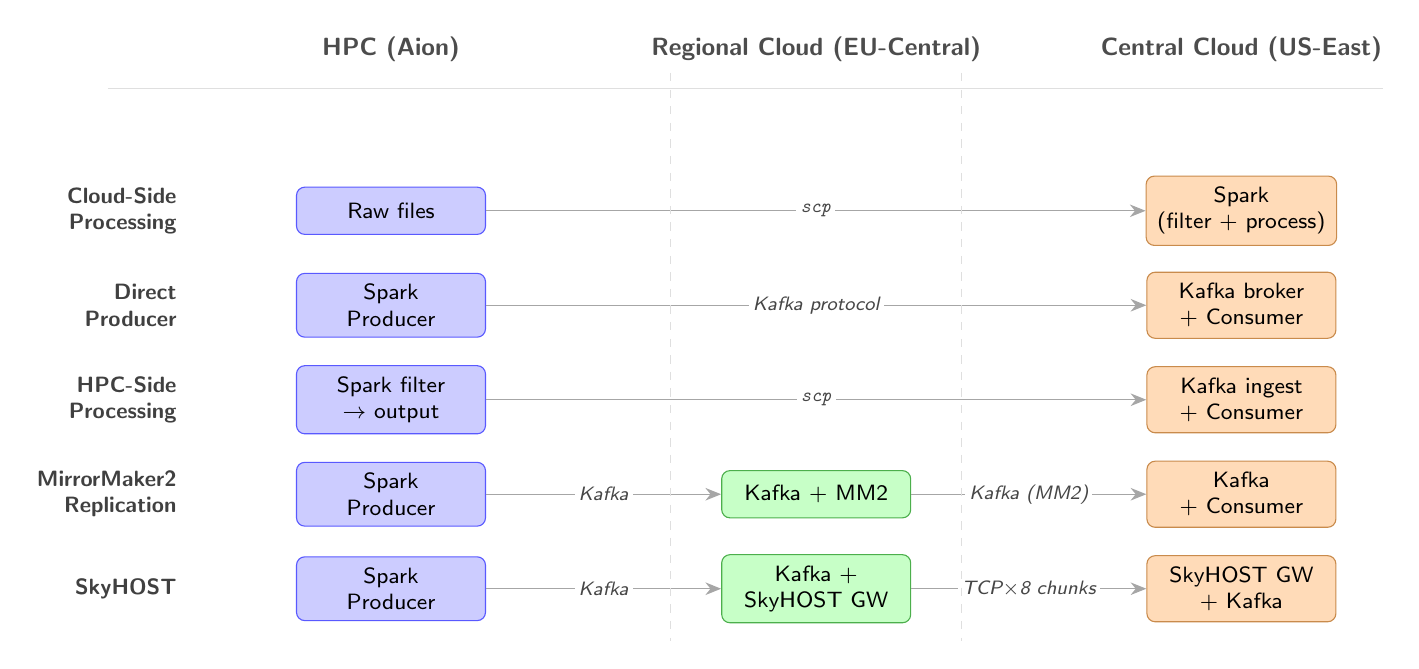
\begin{tikzpicture}[
  font=\sffamily\small,
  every node/.style={font=\sffamily\small},
  box/.style={draw, line width=0.4pt, rounded corners=3pt,
              minimum height=6mm, minimum width=24mm,
              inner sep=4pt, align=center, font=\sffamily\footnotesize},
  hpc/.style={box, fill=blue!20,    draw=blue!65},
  fra/.style={box, fill=green!22,   draw=green!55!black!70},
  use/.style={box, fill=orange!28,  draw=orange!70!black!70},
  wan/.style={-{Stealth[length=2mm,width=1.6mm]}, line width=0.45pt, draw=gray!70},
  arrlbl/.style={font=\sffamily\scriptsize\itshape, text=gray!55!black,
                 inner sep=1.5pt, fill=white},
  rowname/.style={font=\sffamily\footnotesize\bfseries, text=black!75,
                  anchor=east, align=right},
  collbl/.style={font=\sffamily\small\bfseries, text=black!70},
]

% --- column x-coordinates ---
\def\xH{0}
\def\xF{5.4}
\def\xU{10.8}
\def\dy{-1.20}

% --- column headers ---
\node[collbl] at (\xH,0.85) {HPC (Aion)};
\node[collbl] at (\xF,0.85) {Regional Cloud (EU-Central)};
\node[collbl] at (\xU,0.85) {Central Cloud (US-East)};
\draw[gray!25, line width=0.3pt] (-3.6,0.35) -- (12.6,0.35);

% =========================================================
% Row 1 — Cloud-Side Processing
% =========================================================
\node[rowname] at (-2.6, 1*\dy) {Cloud-Side\\Processing};
\node[hpc] (r1h) at (\xH, 1*\dy) {Raw files};
\node[use] (r1u) at (\xU, 1*\dy) {Spark\\(filter + process)};
\draw[wan] (r1h) -- node[arrlbl]{\texttt{scp}} (r1u);

% =========================================================
% Row 2 — Direct Producer
% =========================================================
\node[rowname] at (-2.6, 2*\dy) {Direct\\Producer};
\node[hpc] (r2h) at (\xH, 2*\dy) {Spark\\Producer};
\node[use] (r2u) at (\xU, 2*\dy) {Kafka broker\\+ Consumer};
\draw[wan] (r2h) -- node[arrlbl]{Kafka protocol} (r2u);

% =========================================================
% Row 3 — HPC-Side Processing
% =========================================================
\node[rowname] at (-2.6, 3*\dy) {HPC-Side\\Processing};
\node[hpc] (r3h) at (\xH, 3*\dy) {Spark filter\\$\to$ output};
\node[use] (r3u) at (\xU, 3*\dy) {Kafka ingest\\+ Consumer};
\draw[wan] (r3h) -- node[arrlbl]{\texttt{scp}} (r3u);

% =========================================================
% Row 4 — Kafka-Native Two-Hop
% =========================================================
\node[rowname] at (-2.6, 4*\dy) {MirrorMaker2\\Replication};
\node[hpc] (r4h) at (\xH, 4*\dy) {Spark\\Producer};
\node[fra] (r4f) at (\xF, 4*\dy) {Kafka + MM2};
\node[use] (r4u) at (\xU, 4*\dy) {Kafka\\+ Consumer};
\draw[wan] (r4h) -- node[arrlbl]{Kafka} (r4f);
\draw[wan] (r4f) -- node[arrlbl]{Kafka (MM2)} (r4u);

% =========================================================
% Row 5 — Overlay Two-Hop
% =========================================================
\node[rowname] at (-2.6, 5*\dy) {SkyHOST};
\node[hpc] (r5h) at (\xH, 5*\dy) {Spark\\Producer};
\node[fra] (r5f) at (\xF, 5*\dy) {Kafka +\\SkyHOST GW};
\node[use] (r5u) at (\xU, 5*\dy) {SkyHOST GW\\+ Kafka};
\draw[wan] (r5h) -- node[arrlbl]{Kafka} (r5f);
\draw[wan] (r5f) -- node[arrlbl]{TCP$\times$8 chunks} (r5u);

% --- subtle column dividers ---
\draw[dashed, gray!25, line width=0.3pt] (\xF-1.85, 0.55) -- (\xF-1.85, 5.55*\dy);
\draw[dashed, gray!25, line width=0.3pt] (\xF+1.85, 0.55) -- (\xF+1.85, 5.55*\dy);

\end{tikzpicture}}
\caption{Five HPC-to-Cloud delivery approaches from source to destination. Arrow labels indicate the protocol carried on each WAN segment.}
\label{fig:approaches}
\end{figure}


\section{HPC-to-Cloud Pipeline Evaluation}
\label{sec:bridge}

We evaluate the end-to-end HPC-to-cloud pipeline on a 5\,GB air quality dataset stored on HPC that must be delivered to a destination Kafka broker in us-east-1 after a geographic filter that retains $\sim$11\% of records. We compare five approaches from both batch and streaming paradigms using identical configurations to measure the end-to-end data pipeline time. End-to-end time (E2E) and first-record latency (FRL) are measured from a consumer script on the destination broker. For all five approaches, the timer starts when the pipeline is launched on the source side and stops when the destination consumer observes the first record (FRL) or the last record (E2E). For file-based approaches, this includes the pre-consumer transfer and ingest stages before any destination records become visible.


\subsection{Approaches}

\begin{enumerate}
\item \textbf{Cloud-Side Processing:} The raw dataset is transferred via \texttt{scp} to an EC2 instance in US-East-1, where Spark filters and ingests the result into a local Kafka broker. 

\item \textbf{Direct Producer:} HPC Spark filters the dataset locally and produces filtered records directly to the US-East-1 Kafka broker over WAN.

\item \textbf{HPC-Side Processing:} HPC Spark filters the dataset and writes the output to disk. The filtered file is transferred via \texttt{scp} to the destination, where a Kafka producer ingests it into the local broker.

\item \textbf{MirrorMaker2:} HPC Spark produces the filtered records to a nearby Kafka broker in eu-central-1. MirrorMaker2 then replicates the topic from eu-central-1 to the destination broker in us-east-1.


\item \textbf{SkyHOST:} HPC Spark produces the filtered records to the Kafka broker in eu-central-1. The SkyHOST source gateway consumes from the broker, aggregates records into 32\,MB transport chunks, and transfers via 8 parallel TCP connections to destination gateways that write to the us-east-1 Kafka broker.

\end{enumerate}





\begin{figure}[t]
\centering
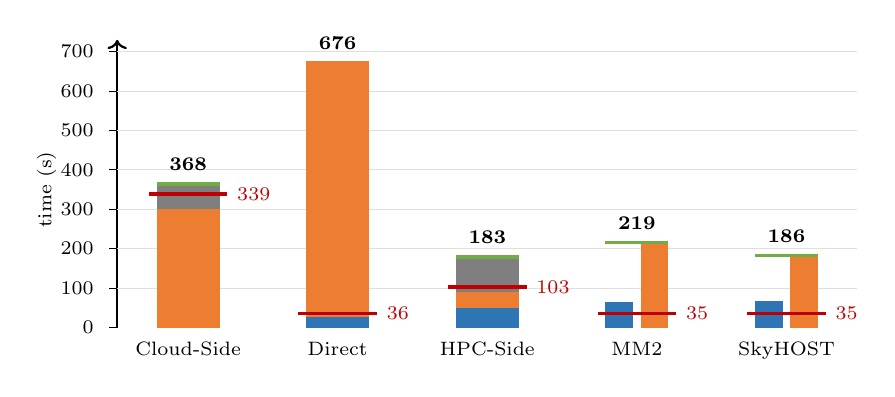
\begin{tikzpicture}[x=1cm, y=0.005cm, font=\footnotesize]

\definecolor{phSpark}{HTML}{2E75B6}
\definecolor{phXfer}{HTML}{ED7D31}
\definecolor{phCloud}{HTML}{7F7F7F}
\definecolor{phCons}{HTML}{70AD47}
\definecolor{frlRed}{HTML}{C00000}

% y-axis
\draw[->, thick] (0.4, 0) -- (0.4, 730);
\foreach \y in {0,100,200,300,400,500,600,700}
  \draw (0.3, \y) -- (0.4, \y) node[left=5pt]{\scriptsize \y};
\node[rotate=90, anchor=south, font=\scriptsize] at (-0.25, 350) {time (s)};

% gridlines
\foreach \y in {100,200,300,400,500,600,700}
  \draw[gray!25, thin] (0.4, \y) -- (9.8, \y);

% ===== Cloud-Side (x=1.3, serial) scp 300 | Spark 59 | drain 9 = 368, FRL=339 =====
\fill[phXfer]  (0.9, 0)    rectangle (1.7, 300);
\fill[phCloud] (0.9, 300)  rectangle (1.7, 359);
\fill[phCons]  (0.9, 359)  rectangle (1.7, 368);
\draw[frlRed, very thick] (0.8, 339) -- (1.8, 339);
\node[frlRed, anchor=west, font=\scriptsize] at (1.8, 339) {339};
\node[anchor=south, font=\scriptsize] at (1.3, 373) {\textbf{368}};
\node[anchor=north, font=\scriptsize] at (1.3, -12) {Cloud-Side};

% ===== Direct (x=3.2, serial-ish) HPC 0-27 | WAN 27-676, FRL=36 =====
\fill[phSpark] (2.8, 0)    rectangle (3.6, 27);
\fill[phXfer]  (2.8, 27)   rectangle (3.6, 676);
\draw[frlRed, very thick] (2.7, 36) -- (3.7, 36);
\node[frlRed, anchor=west, font=\scriptsize] at (3.7, 36) {36};
\node[anchor=south, font=\scriptsize] at (3.2, 681) {\textbf{676}};
\node[anchor=north, font=\scriptsize] at (3.2, -12) {Direct};

% ===== HPC-Side (x=5.1, serial) Spark 50 | scp 41 | ingest 82 | drain 10 = 183, FRL=103 =====
\fill[phSpark] (4.7, 0)    rectangle (5.5, 50);
\fill[phXfer]  (4.7, 50)   rectangle (5.5, 91);
\fill[phCloud] (4.7, 91)   rectangle (5.5, 173);
\fill[phCons]  (4.7, 173)  rectangle (5.5, 183);
\draw[frlRed, very thick] (4.6, 103) -- (5.6, 103);
\node[frlRed, anchor=west, font=\scriptsize] at (5.6, 103) {103};
\node[anchor=south, font=\scriptsize] at (5.1, 188) {\textbf{183}};
\node[anchor=north, font=\scriptsize] at (5.1, -12) {HPC-Side};

% ===== MM2 (x=7.0, overlap: Spark 66 left, Xfer 212 right, drain 7) FRL=35 =====
\fill[phSpark] (6.6, 0)    rectangle (6.95, 66);
\fill[phXfer]  (7.05, 0)   rectangle (7.4, 212);
\fill[phCons]  (6.6, 212)  rectangle (7.4, 219);
\draw[frlRed, very thick] (6.5, 35) -- (7.5, 35);
\node[frlRed, anchor=west, font=\scriptsize] at (7.5, 35) {35};
\node[anchor=south, font=\scriptsize] at (7.0, 224) {\textbf{219}};
\node[anchor=north, font=\scriptsize] at (7.0, -12) {MM2};

% ===== SkyHOST (x=8.9, overlap: Spark 68 left, Xfer 178 right, drain 8) FRL=35 =====
\fill[phSpark] (8.5, 0)    rectangle (8.85, 68);
\fill[phXfer]  (8.95, 0)   rectangle (9.3, 178);
\fill[phCons]  (8.5, 178)  rectangle (9.3, 186);
\draw[frlRed, very thick] (8.4, 35) -- (9.4, 35);
\node[frlRed, anchor=west, font=\scriptsize] at (9.4, 35) {35};
\node[anchor=south, font=\scriptsize] at (8.9, 191) {\textbf{186}};
\node[anchor=north, font=\scriptsize] at (8.9, -12) {SkyHOST};

\end{tikzpicture}

\vspace{6pt}

% ----- Legend (widened so nothing overlaps) -----

\begin{tikzpicture}[font=\scriptsize]
\definecolor{phSpark}{HTML}{2E75B6}
\definecolor{phXfer}{HTML}{ED7D31}
\definecolor{phCloud}{HTML}{7F7F7F}
\definecolor{phCons}{HTML}{70AD47}
\definecolor{frlRed}{HTML}{C00000}
\fill[phSpark] (0, 0)    rectangle (0.3, 0.22);  \node[anchor=west] at (0.35, 0.11) {HPC Spark};
\fill[phXfer]  (2.0, 0)  rectangle (2.3, 0.22);  \node[anchor=west] at (2.35, 0.11) {Transfer};
\fill[phCloud] (3.7, 0)  rectangle (4.0, 0.22);  \node[anchor=west] at (4.05, 0.11) {Cloud process};
\fill[phCons]  (6.1, 0)  rectangle (6.4, 0.22);  \node[anchor=west] at (6.45, 0.11) {Consumer drain};
\draw[frlRed, very thick] (8.7, -0.03) -- (8.7, 0.28);
\node[frlRed, anchor=west] at (8.75, 0.11) {First record};
\end{tikzpicture}

\caption{Phase breakdown and first-record latency (red line) for the 5\,GB pipeline, consumer-measured at the destination broker. Total end-to-end time (s) shown above each bar.}
\label{fig:pipeline_gantt}
\end{figure}


\subsection{Results and Analysis}

Table~\ref{tab:pipeline_results} presents end-to-end time (E2E) and first-record latency (FRL) averaged over 3 runs, and Figure~\ref{fig:pipeline_gantt} decomposes the pipeline into its phases. All runs delivered exactly 9,317,527 records verified via \texttt{kafka-get-offsets} on the destination broker. We analyze the results using two metrics that matter to cloud consumers of HPC pipelines; how quickly the dataset is delivered (E2E), and when the first record becomes available for downstream processing (FRL).

\textit{Batch approaches.} Cloud-Side Processing transfers the raw archive over WAN before filtering and completes in 368\,s, but the first record becomes visible only after \texttt{scp} finishes at 339\,s. HPC-Side Processing pre-filters on HPC, reducing the transfer payload by 89\% before \texttt{scp}, achieving the fastest overall completion at 183\,s. 



\textit{Streaming approaches.} Direct Producer writes filtered records directly from HPC Spark to the us-east-1 Kafka broker over WAN and is bounded by the per-partition acknowledgment cycle, completing in 676\,s. MirrorMaker~2 routes through a regional broker in eu-central-1 and replicates cross-region at 8.54\,MB/s, with HPC Spark overlapping the transfer and completing in 219\,s. 

\begin{table}[t]
\centering
\caption{HPC-to-cloud pipeline end-to-end time and first-record latency (s) for the 5\,GB dataset, averaged over 3 runs, measured by a consumer script on the destination broker. All approaches deliver 9{,}317{,}527 records, verified via \texttt{kafka-get-offsets}.}
\label{tab:pipeline_results}
\small
\begin{tabular*}{0.65\textwidth}{@{\extracolsep{\fill}}clcrr@{}}
\toprule
\textbf{\#} & \textbf{Approach} & \textbf{Type} & \textbf{E2E (s)} & \textbf{FRL (s)} \\
\midrule
1 & Cloud-Side Processing & Batch   & 368 & 339 \\
2 & Direct Producer       & Stream  & 676 &  36 \\
3 & HPC-Side Processing   & Batch   & 183 & 103 \\
4 & MM2 Replication       & Stream  & 219 &  35 \\
5 & SkyHOST               & Stream  & 186 &  35 \\
\bottomrule
\end{tabular*}
\end{table}



SkyHOST shares the same first hop as MM2 but replaces the cross-region Kafka protocol with transport-layer chunking. Source gateways aggregate records into 32\,MB chunks and deliver them over 8 parallel TCP connections, sustaining 10.7\,MB/s and completing in 186\,s. Both two-hop streaming approaches deliver the first record within 35\,s because HPC-side production, cross-region transfer, and destination ingestion execute concurrently. 


Direct Producer achieves similar first-record latency (36\,s) to the two-hop approaches (35\,s). This is because FRL is dominated by Spark startup ($\sim$27\,s), and all three streaming approaches expose records as soon as Spark emits its first micro-batch. The difference in performance becomes apparent for sustained throughput since Direct pays the full HPC-to-us-east-1 acknowledgment cycle for every Kafka batch. In contrast, MM2 and SkyHOST decouple the producer from the WAN by writing first to a nearby regional broker, and then move the long-haul transfer into a separate downstream stage. The lower-RTT first hop and the higher-quality intra-cloud backbone improve sustained throughput even though the logical path contains two hops.


Batch and streaming approaches show different strengths depending on the workload. HPC-Side Processing achieves the lowest end-to-end time but enforces a strict serial pipeline in which filtered data must be written to HPC disk, transferred via \texttt{scp}, and re-ingested into destination Kafka. However, in the HPC-Side Processing approach, no records reach a cloud consumer until all three phases are complete, and the first-record latency (FRL) is 103\,s for the 5\,GB dataset. When incremental data availability is required for continuous reprocessing jobs or concurrent cloud consumers, a streaming approach becomes necessary.

SkyHOST maintains an end-to-end streaming pipeline in which all stages overlap, as Spark produces records to the eu-central-1 broker while filtering, SkyHOST gateways consume and forward them in transport-layer chunks, and destination gateways write to us-east-1 Kafka. First records reach the destination within $\sim$35\,s, 3$\times$ faster than the batch approach. This pipelined architecture works better for recurring workloads: when HPC jobs run on a schedule, SkyHOST delivers records continuously, whereas the file-based approach forces consumers to wait for each complete write-transfer-ingest cycle. 

In exchange, the first record arrives 3$\times$ earlier (35\,s vs.\ 103\,s) and remains bounded by pipeline startup rather than transfer time. Against the industry-standard MM2 baseline with identical regional routing and BBR tuning, SkyHOST is 15\% faster end-to-end (186\,s vs.\ 219\,s) with the same FRL. For one-time archival delivery, HPC-Side Processing's write-transfer-ingest pipeline remains a reasonable choice. For the recurring workloads motivated in Section~\ref{sec:related}, where scheduled HPC jobs feed continuous cloud consumers, batch delivery forces each consumer to wait for a full cycle before any data becomes visible. SkyHOST preserves streaming semantics end-to-end, matches batch completion, and decouples first-record latency from transfer duration.


\section{Discussion and Guidelines}
\label{sec:discussion}

Spark-Kafka achieves 72--180\,MB/s throughput for pre-filtering large archives on HPC. The cross-region transfer bridge (8.5--10.7\,MB/s) becomes the bottleneck, bounded by Kafka's protocol overhead and WAN latency. SkyHOST achieves 10.7\,MB/s and MM2 reaches 8.54\,MB/s with TCP tuning (BBR, 128\,MB buffers) for cross-region transfer. Direct Kafka production remains an order of magnitude slower than the routed approaches.

Our findings yield four practical guidelines. First, Spark pre-filtering on HPC provides 89\% data reduction before transfer, yielding larger end-to-end speedups. Second, routing through a nearby regional cloud with a low-latency regional broker achieves 11--20$\times$ higher throughput than direct long-distance production. Third, TCP tuning with BBR congestion control and large socket buffers is essential for cross-region Kafka transfers to improve throughput. Fourth, HPC network capabilities remain underutilized as our peak 180\,MB/s uses only 14\% of 10\,Gbps Ethernet, motivating RDMA-native alternatives. Based on our comprehensive evaluation, Table~\ref{tab:guidelines} provides practical recommendations for different deployment objectives.

\begin{table}[t]
\centering
\caption{Configuration guidelines for Spark-Kafka across the computing continuum.}
\label{tab:guidelines}
\small
\begin{tabular}{@{}p{3.8cm}p{5.8cm}r@{}}
\toprule
\textbf{Objective} & \textbf{Recommended Configuration} & \textbf{Performance} \\
\midrule
Max HPC throughput & 4--8 part., Spark Streaming, 16KB batch & $\sim$180\,MB/s \\
HPC with replication & RF=3, acks=1, $\geq$4 partitions & $\sim$102\,MB/s \\
HPC with durability & RF=3, acks=all, 8 partitions & $\sim$62\,MB/s \\
HPC$\to$cloud (batch) & Pre-filter + scp filtered data & 183\,s / 5\,GB \\
HPC$\to$cloud (stream) & 2-hop regional + SkyHOST + BBR & 186\,s / 5\,GB \\
\bottomrule
\end{tabular}
\end{table}

\textbf{Limitations.} We evaluate a single HPC cluster (Aion) with Kafka~2.8 and at most 3 brokers. HPC-to-cloud experiments use one dataset scale (5\,GB); smaller datasets may exhibit higher fixed-overhead fractions. We ran the experiment for fixed regions (Luxembourg--Frankfurt--Virginia), results may vary for other regions, cross-cloud, and different cloud instance types.




\section{Conclusion}
\label{sec:conclusion}

We presented a comprehensive evaluation of containerized Spark-Kafka streaming on HPC and five end-to-end approaches for delivering HPC processed data to the cloud. Spark Structured Streaming achieves up to 180\,MB/s throughput, and RF=3 with \texttt{acks=1} provides data replication at negligible throughput cost across 240 configurations on the HPC cluster. 

For HPC-to-cloud delivery, we compared five strategies on a 5\,GB dataset, and calculated the end-to-end pipeline transfer time across all approaches. Our results show that streaming does not need to sacrifice completion time to preserve incremental data availability. HPC-side batch processing is the fastest overall at 183\,s E2E transfer, but no destination record becomes visible until 103\,s. 

Direct Kafka over WAN is throttled by the per-partition acknowledgment cycle and requires 676\,s. MirrorMaker~2 and SkyHOST both route through a regional broker and expose the first record within 35\,s, 3$\times$ earlier than batch. SkyHOST further replaces the cross-region Kafka protocol with transport-layer batching, sustaining 10.7\,MB/s and completing in 186\,s, within 2\% of the fastest batch approach and 15\% faster than MM2 (219\,s). Ultimately, HPC pre-filtering combined with optimized Kafka transport provides an efficient, end-to-end streaming path from HPC to the cloud. Future work will extend to dynamic pipeline adaptation, larger-scale deployments, and cross-cloud architectures for recurring streaming data workflows.


\bibliographystyle{splncs04}
\begin{thebibliography}{21}

\bibitem{varghese2018next}
Varghese, B., Buyya, R.: Next generation cloud computing: New trends and research directions. Future Gener.\ Comput.\ Syst.\ 79, 849--861 (2018)

\bibitem{buyya2018manifesto}
Buyya, R., et al.: A manifesto for future generation cloud computing. ACM Comput.\ Surv.\ \textbf{51}(5), 1--38 (2018)

\bibitem{karimov2018benchmarking}
Karimov, J., et al.: Benchmarking distributed stream data processing systems. In: Proc.\ IEEE ICDE, pp.\ 1507--1518 (2018)

\bibitem{lopez2016performance}
Lopez, M.A., et al.: A performance comparison of open-source stream processing platforms. In: Proc.\ IEEE GLOBECOM, pp.\ 1--6 (2016)

\bibitem{chintapalli2016benchmarking}
Chintapalli, S., et al.: Benchmarking streaming computation engines. In: Proc.\ IEEE IPDPS Workshops, pp.\ 1789--1792 (2016)

\bibitem{kulkarni2025sprobench}
Kulkarni, A.D., Ghiasvand, S.: SProBench: Stream processing benchmark for HPC infrastructure. In: Proc.\ Euro-Par, LNCS, vol.\ 15902, pp.\ 268--282 (2025)


\bibitem{armbrust2018structured}
Armbrust, M., et al.: Structured Streaming: A declarative API for real-time applications in Apache Spark. In: Proc.\ ACM SIGMOD, pp.\ 601--613 (2018)

\bibitem{varrette2014management}
Varrette, S., et al.: Management of an academic HPC cluster: The UL experience. In: Proc.\ HPCS, pp.\ 959--966 (2014)

\bibitem{tariq2026skyhost}
Tariq, M.A., Danoy, G., Bouvry, P.: SkyHOST: A unified architecture for cross-cloud hybrid object and stream transfer. arXiv preprint arXiv:2603.20512 (2026).


\bibitem{mofka2023}
Dorier, M., et al.: Toward a persistent event-streaming system for HPC applications. Front.\ High Perform.\ Comput.\ (2025)

\bibitem{mm2kafka}
Apache Software Foundation: KIP-382: MirrorMaker 2.0. Apache Kafka Improvement Proposals (2019)

\bibitem{ds2hpc2025}
George, A., et al.: From edge to HPC: Investigating cross-facility data streaming architectures. In: Proc.\ SC Workshops (INDIS) (2025)

\bibitem{pilotstreaming2018}
Luckow, A., et al.: Pilot-Streaming: A stream processing framework for HPC. In: Proc.\ IEEE eScience, pp.\ 177--188 (2018)


\bibitem{datacloud2023}
Plociennik, M., et al.: DataCloud: Enabling the big data pipelines lifecycle on the computing continuum. In: Proc.\ IEEE BigData, pp.\ 3130--3139 (2023)

\bibitem{balouek2019continuum}
Balouek-Thomert, D., et al.: Towards a computing continuum: Enabling edge-to-cloud integration for data-driven workflows. Int.\ J.\ High Perform.\ Comput.\ Appl.\ \textbf{33}(6), 1159--1174 (2019)

\bibitem{miller2023iri}
Miller, W.L., et al.: Integrated Research Infrastructure Architecture Blueprint Activity (Final Report). U.S. DOE Office of Science, LBNL (2023)

\bibitem{hersbach2020era5}
Hersbach, H., et al.: The ERA5 global reanalysis. Q.\ J.\ R.\ Meteorol.\ Soc.\ \textbf{146}(730), 1999--2049 (2020)

\bibitem{extract2023}
EXTRACT Consortium: A distributed data-mining software platform for extreme data across the compute continuum. EU Horizon Project 101093110 (2023--2026)

\bibitem{lclstream2025}
Esposito, C., et al.: The LCLStream ecosystem for multi-institutional dataset exploration. In: Proc.\ SCA/HPCAsia Workshops (2026)

\bibitem{catch}
Monti, H.M., Butt, A.R., Vazhkudai, S.S.: CATCH: A cloud-based adaptive data transfer service for HPC. In: 2011 IEEE International Parallel \& Distributed Processing Symposium, pp.\ 1242--1253. IEEE (2011)


\end{thebibliography}

\end{document}
